\documentclass[10pt,a4paper]{article}

% --- Core Packages ---
\usepackage[utf8]{inputenc}
\usepackage[T1]{fontenc}
\usepackage{lmodern}
\usepackage[margin=1.2cm, top=1.4cm, bottom=0.9cm, headheight=18pt, headsep=10pt]{geometry}
\usepackage{graphicx}
\usepackage{fancyhdr}
\usepackage{hyperref}
\usepackage{tabularx}
\usepackage{subcaption}
\usepackage{etoolbox}
\usepackage{xcolor}

% --- Load Student & Course Metadata ---
\IfFileExists{student-infom.tex}{%
  \input{student-infom.tex}%
}{%
  % ==============================================================================
% FALLBACK / TEMPLATE STUDENT & COURSE INFORMATION (Git-Tracked)
% ==============================================================================
% Faculty and Department Information
\newcommand{\facultyName}{Faculty of Engineering}
\newcommand{\departmentName}{Department of Computer Engineering}

% Course and Academic Term Information
\newcommand{\courseCode}{BIM493}
\newcommand{\courseName}{Mobile Programming I}
\newcommand{\academicTerm}{Fall 2026--2027}

% Student Credentials (Template / Placeholder)
\newcommand{\studentOneName}{Student One}
\newcommand{\studentOneId}{123456}

\newcommand{\studentTwoName}{Student Two}
\newcommand{\studentTwoId}{654321}

% Default GitHub Repository Link (Points to GitHub homepage)
\newcommand{\repositoryUrl}{https://github.com}
%
}

% --- Assignment Metadata ---
\newcommand{\assignmentNumber}{Assignment \#1}
\newcommand{\assignmentTitle}{Campus Event Explorer}

% --- Subtle Formal Colors ---
\definecolor{headergray}{gray}{0.5}
\definecolor{linegray}{gray}{0.7}
\definecolor{linkblue}{rgb}{0,0.2,0.6}

% --- Hyperlink Setup ---
\hypersetup{
    colorlinks=true,
    linkcolor=black,
    urlcolor=linkblue,
    citecolor=black,
    pdftitle={\courseCode\ - \assignmentNumber},
    pdfauthor={\studentOneName}
}

% --- Page Header (Course on left, Academic Term on right) ---
\pagestyle{fancy}
\fancyhf{}
\fancyhead[L]{\small \textbf{\courseCode: \courseName}}
\fancyhead[R]{\small \color{headergray}\academicTerm}
\renewcommand{\headrulewidth}{0.4pt}
\fancyfoot{}

% Image search path
\graphicspath{{./}{../screenshots/}}

\begin{document}

% ==============================================================================
% 1. INSTITUTIONAL LOGO & TITLE (Clean, Centered, Relaxed)
% ==============================================================================
\begin{center}
    \IfFileExists{estu_logo.png}{%
        
\includegraphics[height=3.7cm]{estu_logo.png}\\[0.25cm]
    }{}
    {\normalsize \facultyName\ \ --- \ \ \departmentName}\\[0.2cm]
    {\LARGE \textbf{\assignmentTitle}}\\[0.15cm]
    {\normalsize \assignmentNumber\ Technical Submission Report}\\[0.2cm]
\end{center}

\vspace{0.1cm}
\hrule height 0.4pt
\vspace{0.25cm}

% ==============================================================================
% 2. STUDENT & REPOSITORY METADATA (Stacked Vertically, Unconstrained)
% ==============================================================================
\noindent
\small
\begin{tabularx}{\textwidth}{@{} l X @{}}
    \textbf{Student 1:} & \studentOneName\ (\studentOneId) \\[3pt]
    \ifdefempty{\studentTwoName}{}{%
        \textbf{Student 2:} & \studentTwoName\ (\studentTwoId) \\[3pt]
    }
    \textbf{Repository:} & \href{\repositoryUrl}{\nolinkurl{\repositoryUrl}} \\[3pt]
    \textbf{Execution (Bash / CMD):} & \texttt{cd 01-campus-event-explorer \&\& flutter run} \\[3pt]
    \textbf{Execution (PowerShell):} & \texttt{cd 01-campus-event-explorer; flutter run} \\
\end{tabularx}

\vspace{0.2cm}
\hrule height 0.4pt
\vspace{0.35cm}

% ==============================================================================
% 3. APPLICATION SCREENSHOTS (System Evidence Grid)
% ==============================================================================
\begin{figure}[h!]
    \centering
    % Row 1
    \begin{subfigure}[b]{0.31\textwidth}
        \centering
        \fboxsep=0pt\fboxrule=0.4pt\fbox{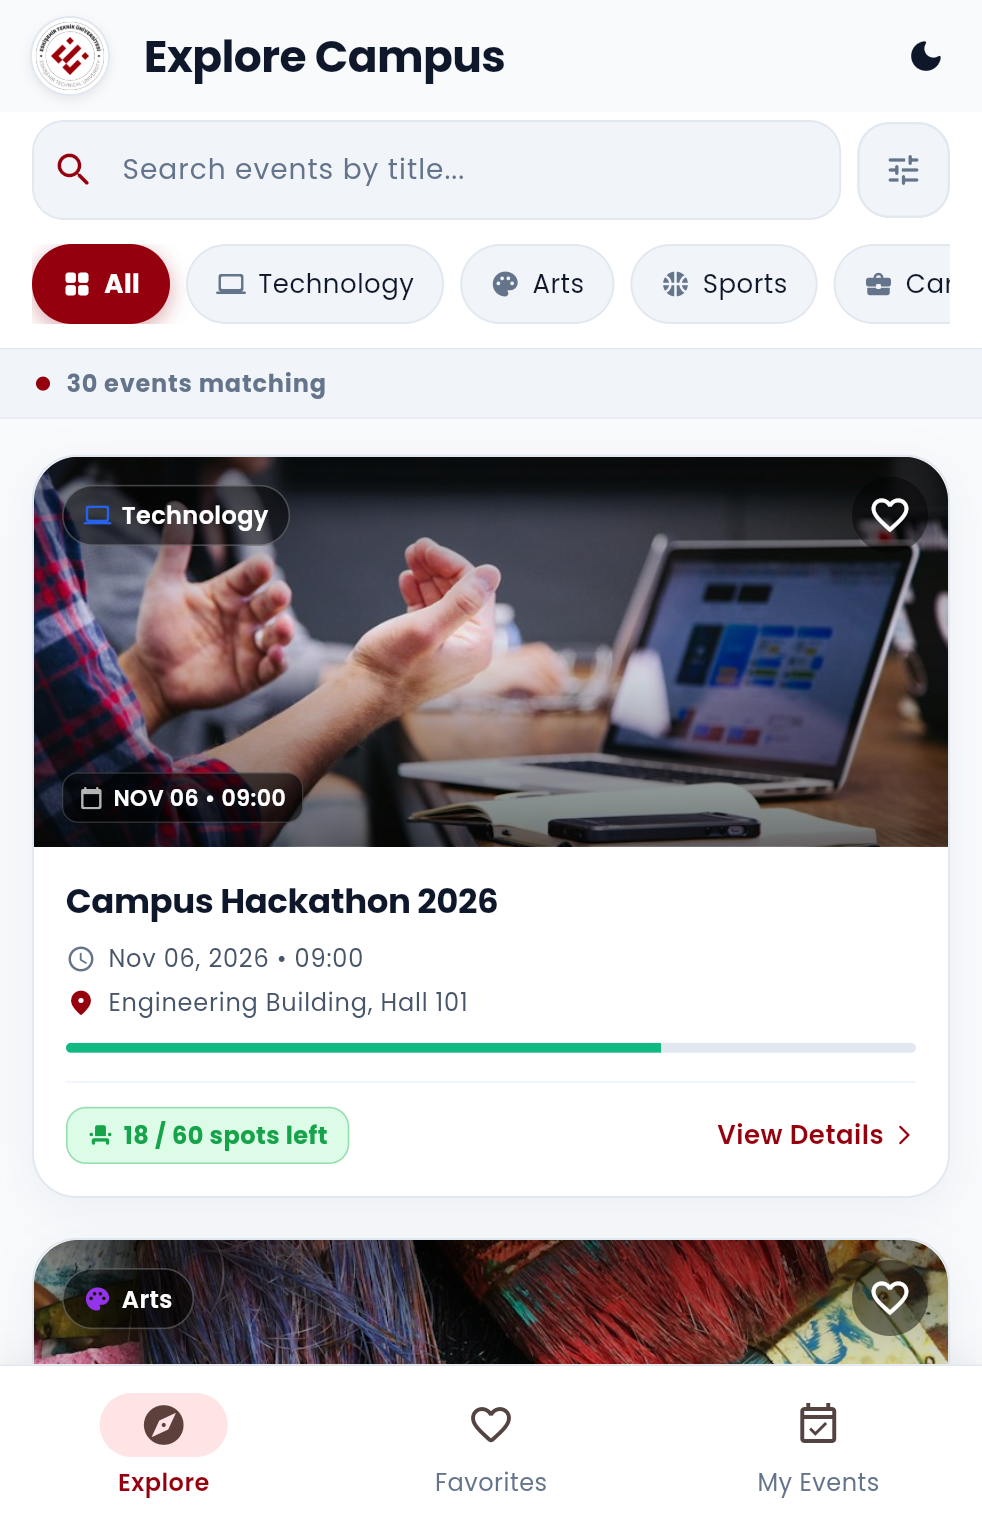
\includegraphics[height=6.1cm]{assignment1_01_explore_overview.png}}\\[4pt]
        {\footnotesize\textbf{Figure 1:} Explore Overview}
    \end{subfigure}
    \hfill
    \begin{subfigure}[b]{0.31\textwidth}
        \centering
        \fboxsep=0pt\fboxrule=0.4pt\fbox{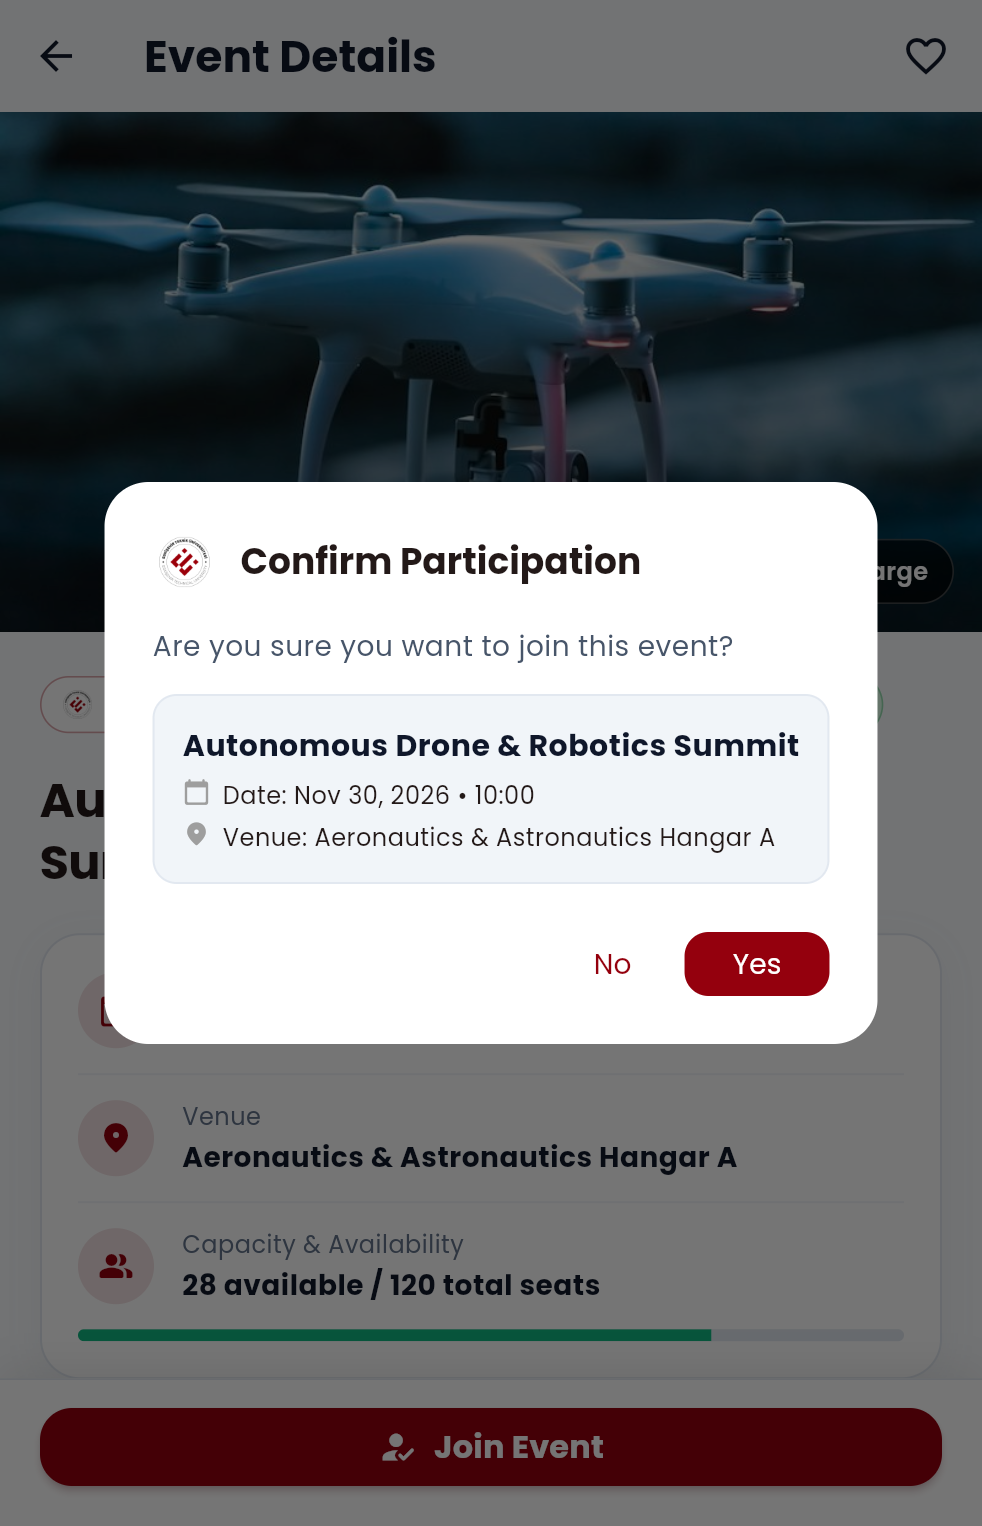
\includegraphics[height=6.1cm]{assignment1_02_event_details_dialog.png}}\\[4pt]
        {\footnotesize\textbf{Figure 2:} Event Details \& Participation}
    \end{subfigure}
    \hfill
    \begin{subfigure}[b]{0.31\textwidth}
        \centering
        \fboxsep=0pt\fboxrule=0.4pt\fbox{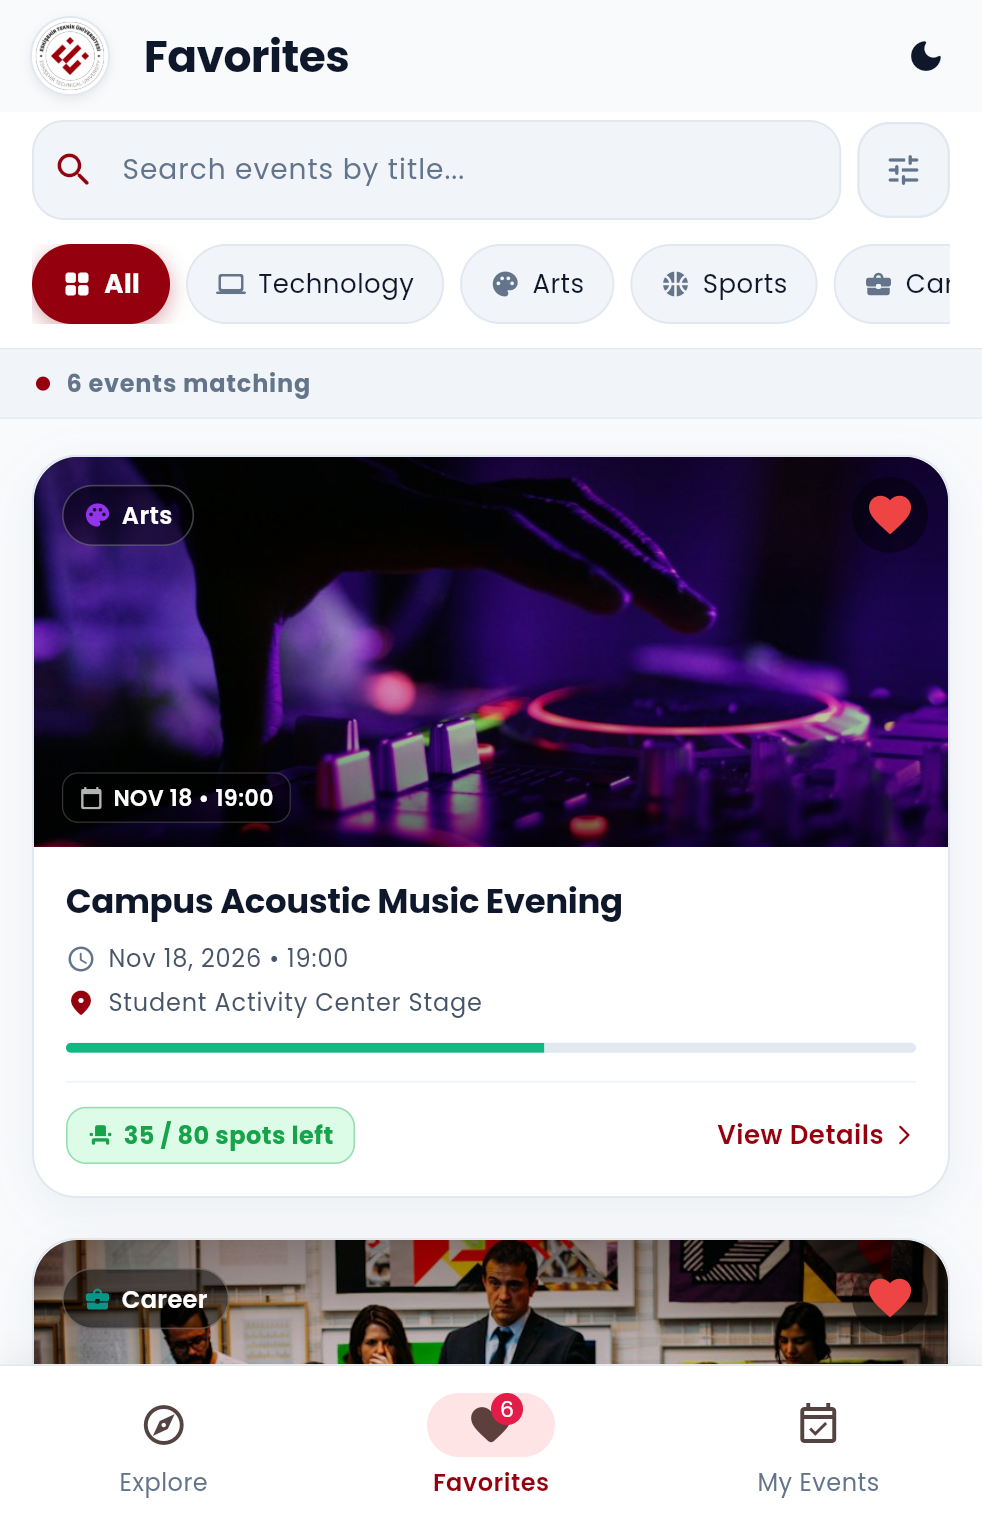
\includegraphics[height=6.1cm]{assignment1_03_favorites_collection.png}}\\[4pt]
        {\footnotesize\textbf{Figure 3:} Favorites Collection}
    \end{subfigure}

    \vspace{0.3cm}

    % Row 2
    \begin{subfigure}[b]{0.31\textwidth}
        \centering
        \fboxsep=0pt\fboxrule=0.4pt\fbox{
\includegraphics[height=6.1cm]{assignment1_04_sort_bottom_sheet.png}}\\[4pt]
        {\footnotesize\textbf{Figure 4:} Sorting Modal Sheet}
    \end{subfigure}
    \hfill
    \begin{subfigure}[b]{0.31\textwidth}
        \centering
        \fboxsep=0pt\fboxrule=0.4pt\fbox{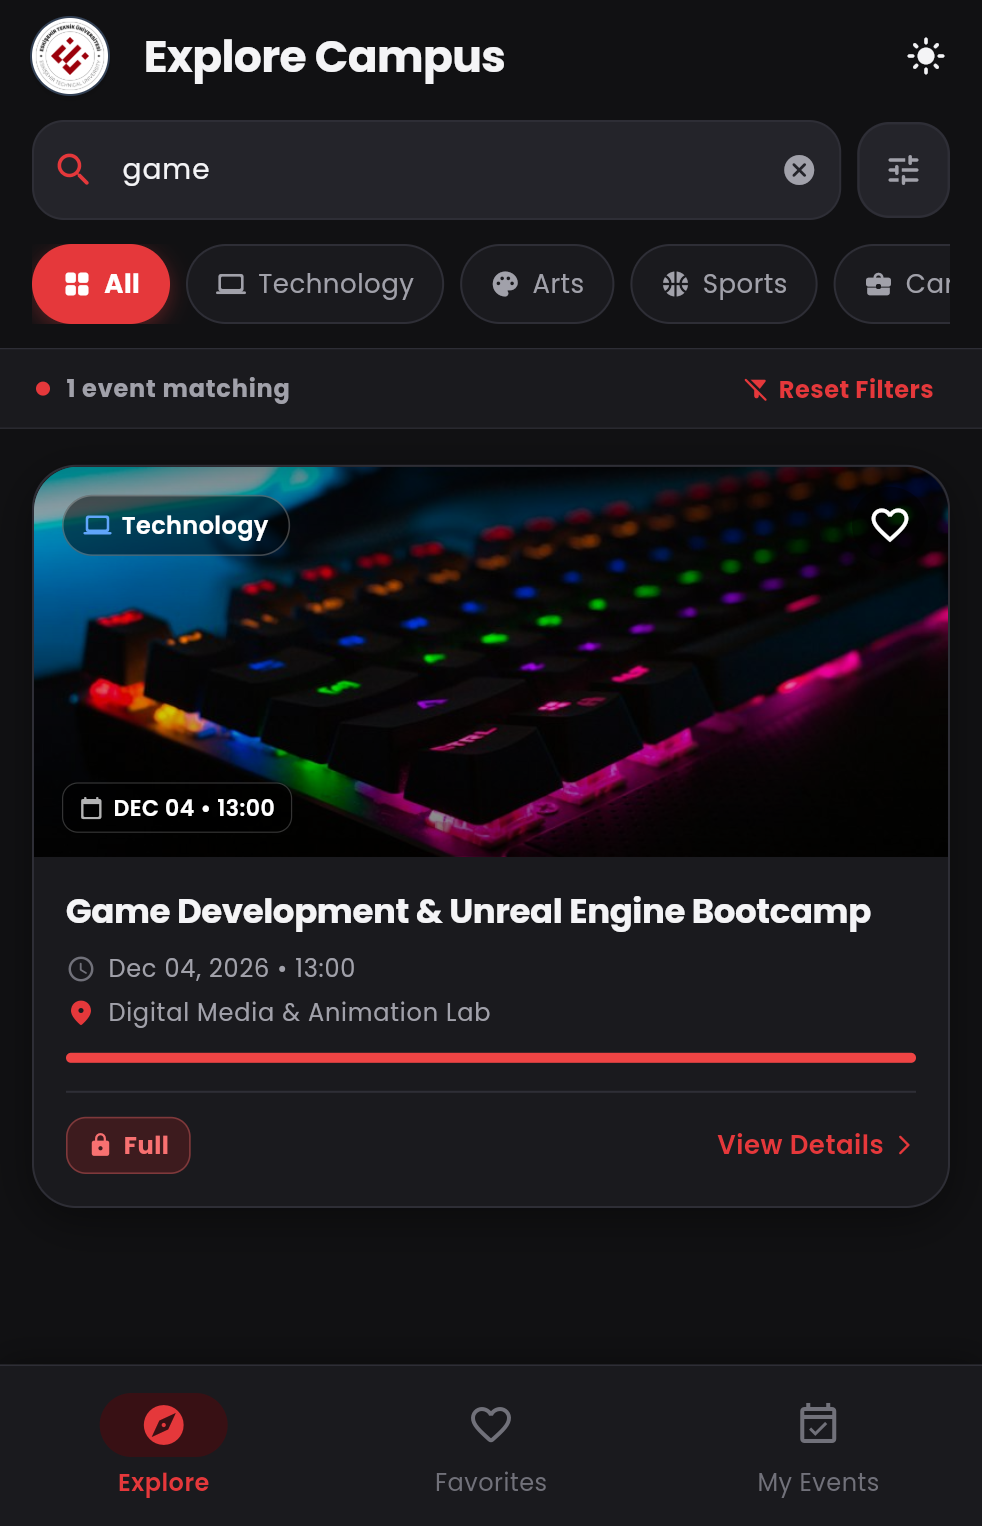
\includegraphics[height=6.1cm]{assignment1_05_search_dark_mode.png}}\\[4pt]
        {\footnotesize\textbf{Figure 5:} Filtered Search \& Dark Theme}
    \end{subfigure}
    \hfill
    \begin{subfigure}[b]{0.31\textwidth}
        \centering
        \fboxsep=0pt\fboxrule=0.4pt\fbox{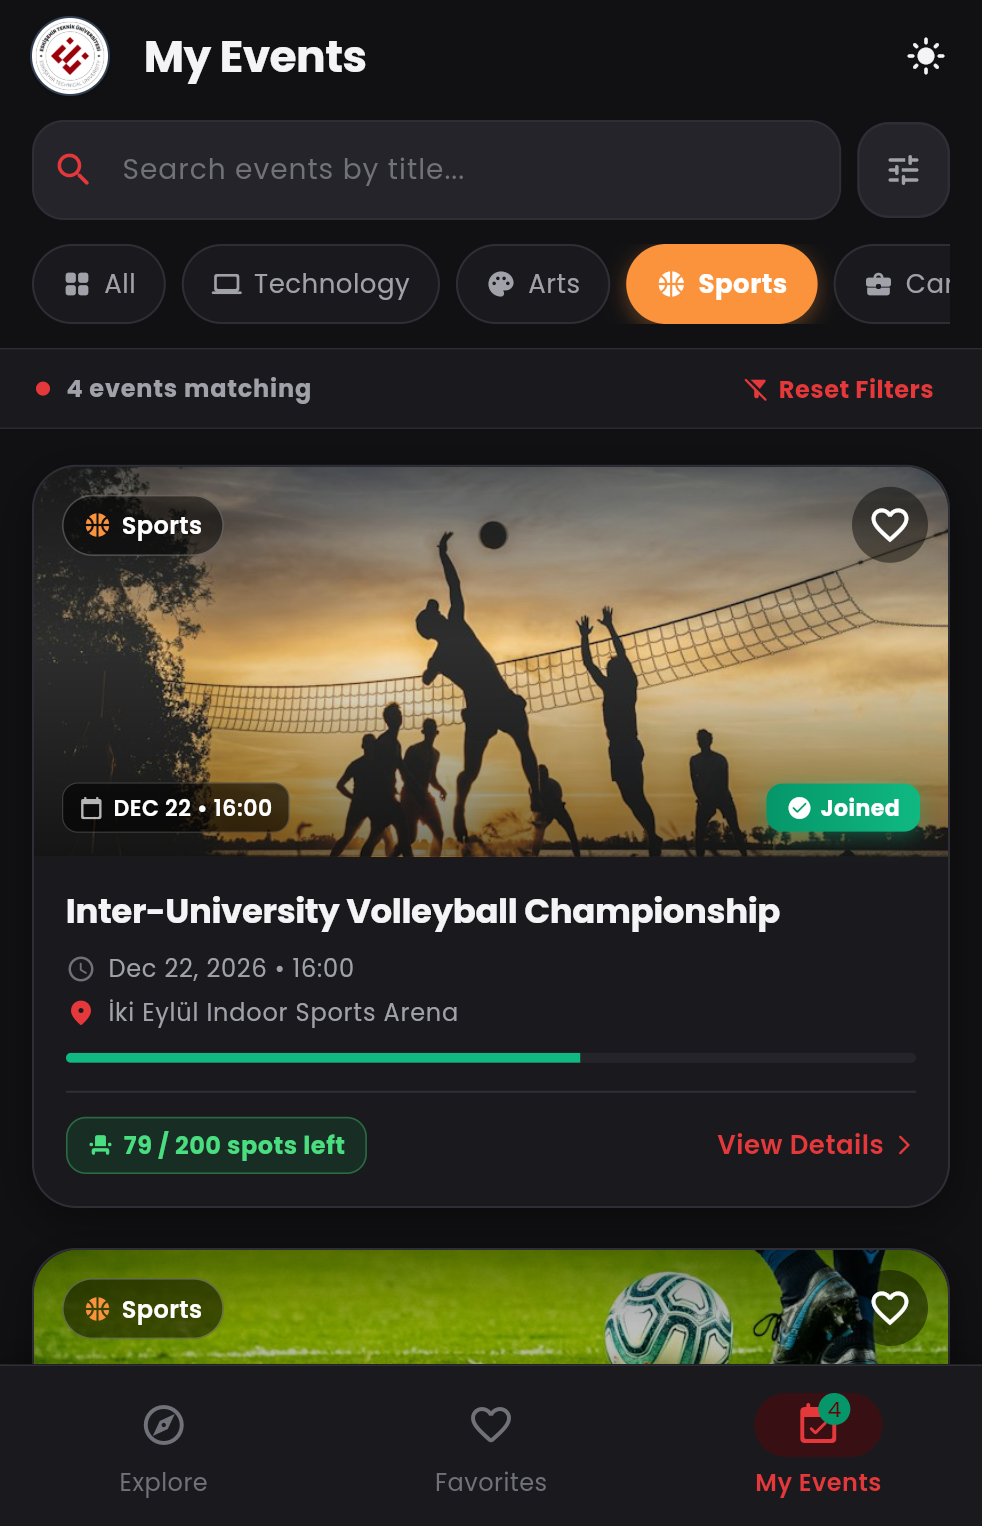
\includegraphics[height=6.1cm]{assignment1_06_my_events_sports_dark.png}}\\[4pt]
        {\footnotesize\textbf{Figure 6:} My Events}
    \end{subfigure}
\end{figure}

\vspace{0.2cm}
\hrule height 0.4pt
\vspace{0.15cm}
\noindent
{\scriptsize \textbf{Environment Version (\texttt{flutter --version}):}}\\[1pt]
{\fontsize{6.2pt}{7.5pt}\selectfont\ttfamily
Flutter 3.47.7 $\cdot$ channel stable $\cdot$ \url{https://github.com/flutter/flutter.git}\\
Framework $\cdot$ revision abaf9c5237 (5 days ago) $\cdot$ 2026-10-08 09:51:21 -0700\\
Engine $\cdot$ hash d8a2d6c768c334d53e16277f837970ffa1e2de81 (revision deb287481e)\\
Tools $\cdot$ Dart 3.13.5 $\cdot$ DevTools 2.60.0\par
}

\end{document}
